\newpage % Rozdziały zaczynamy od nowej strony.
\section{Wstep teoretyczny}

% # TODO: Zamienić obrazki definicji klasyfikacji i segmentacji na te z mojego zbioru

\subsection{Nadzorowane uczenie maszynowe}
Uczenie maszynowe to podzbiór sztucznej inteligencji, który obejmuje rozwój algorytmów i modeli statystycznych, które umożliwiają komputerom uczenie się z danych, bez wyraźnego programowania. Jest to metoda uczenia komputerów, aby rozpoznawały wzorce i dokonywały przewidywań na ich podstawie.

Uczenie nadzorowane to rodzaj uczenia maszynowego, w którym algorytm jest szkolony na etykietowanym zestawie danych, gdzie pożądane wyjście dla danego wejścia jest już znane. W kontekście głębokiego uczenia się, algorytmy uczenia nadzorowanego wykorzystują sieci neuronowe do uczenia się z danych i dokonywania przewidywań.

Jedną z głównych zalet wykorzystania głębokiego uczenia do uczenia nadzorowanego jest możliwość uczenia się złożonych i nieliniowych zależności z danych. Głębokie sieci neuronowe, z ich wieloma warstwami, mogą uczyć się i reprezentować wielowymiarowe i abstrakcyjne cechy danych, co pozwala im osiągnąć satysfakcjonujące rezultaty w wielu zadaniach. Dodatkowo, algorytmy głębokiego uczenia mogą obsługiwać duże ilości danych i mogą być łatwo zrównoleglone, co pozwala na skrócenie czasu treningu.

Istnieją jednak również ograniczenia w stosowaniu głębokiego uczenia do uczenia nadzorowanego. Jednym z ograniczeń jest konieczność posiadania dużej ilości oznaczonych danych. Aby wytrenować głęboką sieć neuronową, wymagana jest znaczna ilość oznaczonych danych, które nie zawsze mogą być łatwo dostępne lub łatwe do uzyskania. Dodatkowo, algorytmy głębokiego uczenia mogą być podatne na przepełnienie, zwłaszcza gdy ilość danych jest ograniczona. Może to prowadzić do słabej generalizacji na niewidzianych danych.
\subsection{Głębokie uczenie i konwolucje}
Uczenie głębokie odnosi się do podzbioru uczenia maszynowego, które charakteryzuje się wykorzystaniem głębokich sieci neuronowych, które składają się z wielu warstw sztucznych neuronów. W kontekście wizji komputerowej, głębokie uczenie zostało wykorzystane do osiągnięcia wielu sukcesów w szerokim zakresie zadań, w tym klasyfikacji obrazów, wykrywania obiektów i segmentacji semantycznej.

Jedną z kluczowych zalet głębokiego uczenia w wizji komputerowej jest zdolność do automatycznego uczenia się hierarchicznych reprezentacji obrazów, które mogą być wykorzystane do wyodrębnienia wysokopoziomowych cech, które są wysoce zróżnicowane dla danego zadania. Stanowi to kontrast do tradycyjnych metod widzenia komputerowego, które zazwyczaj opierają się na ręcznie opracowanych cechach, które są zaprojektowane tak, aby były informatywne dla konkretnego zadania.

Uczenie głębokie, a konkretnie głębokie konwolucyjne sieci neuronowe (CNN), zostały szeroko zaadoptowane w dziedzinie widzenia komputerowego, z wieloma sukcesami w różnych zadaniach, takich jak klasyfikacja obrazów, wykrywanie obiektów i segmentacja semantyczna. W tym rozdziale zostanie przedstawiony krótki przegląd niektórych najważniejszych kamieni milowych w rozwoju głębokich CNN dla wizji komputerowej, ze szczególnym uwzględnieniem klasyfikacji obrazów, jako zadania, którego rozwój przyczynił się do znacznego rozrostu wiedzy wsród innych zadań.

Jedną z najwcześniejszych i najbardziej wpływowych prac w dziedzinie głębokich CNN dla wizji komputerowej jest "ImageNet Classification with Deep Convolutional Neural Networks" autorstwa Alexa Krizhevsky'ego, Ilya Sutskevera i Geoffrey'a Hintona (2012). W pracy tej przedstawiono zastosowanie głębokich sieci neuronowych do klasyfikacji obrazów i osiągnięto najwyższej wyniki na zbiorze danych ImageNet. Praca ta wyznaczyła nowy punkt odniesienia dla klasyfikacji obrazów i zapoczątkowała szerokie zastosowanie CNN w zadaniach widzenia komputerowego.

W kolejnych latach wielu badaczy zaproponowało różne modyfikacje i ulepszenia podstawowej architektury CNN. Jednym z ważnych wkładów jest architektura Inception, wprowadzona przez Szegedy i in. w "Going Deeper with Convolutions" (2014). Architektura Inception wykorzystuje kombinację różnych rozmiarów filtrów konwolucyjnych do ekstrakcji cech w wielu skalach, co pozwala sieci uczyć się bardziej złożonych i abstrakcyjnych cech niż wcześniejsze architektury.

Kolejną kluczową innowacją w rozwoju głębokich CNN dla wizji komputerowej jest wykorzystanie połączeń rezydualnych, które zostało zaproponowane przez He i in. w "Deep Residual Learning for Image Recognition" (2016). Połączenia rezydualne pozwalają na trenowanie bardzo głębokich sieci poprzez ułatwienie optymalizacji gradientów i zapobieganie problemowi znikającego gradientu. Architektura ResNet, która wykorzystuje połączenia rezydualne, wykazała, że osiąga lepszą wydajność w zadaniu klasyfikacji ImageNet niż poprzednie architektury.

Podsumowując, głębokie CNN są wysoce efektywne w zadaniach widzenia komputerowego, takich jak klasyfikacja obrazów. Rozwój głębokich CNN zaznaczył się kilkoma ważnymi kamieniami milowymi, w tym wykorzystaniem głębokich architektur, różnych architektur, takich jak Inception, oraz wykorzystaniem połączeń rezydualnych. Te innowacje doprowadziły do znacznej poprawy wydajności na zbiorze danych ImageNet i zainspirowały dalsze badania w innych zadaniach widzenia komputerowego.
\subsection{Segmentacja semantyczna}
Segmentacja semantyczna jest zadaniem w wizji komputerowej, które ma na celu przypisanie semantycznej etykiety do każdego piksela w obrazie. Zadanie to ma wiele praktycznych zastosowań, takich jak rozumienie sceny, wykrywanie obiektów i edycja obrazów. W tym rozdziale przedstawimy przegląd niektórych najważniejszych kamieni milowych w rozwoju głębokich splotowych sieci neuronowych (CNN) do segmentacji semantycznej, analizując kluczowe prace w tej dziedzinie.

Jednym z najwcześniejszych i najbardziej wpływowych artykułów w dziedzinie głębokich CNN do segmentacji semantycznej jest "Fully Convolutional Networks for Semantic Segmentation" autorstwa Longa, Shelhamera i Darrella (2015)\cite{fcn}. W pracy tej, zaprezentowanej na konferencji Computer Vision and Pattern Recognition (CVPR), przedstawiono architekturę sieci w pełni splotową (FCN) do segmentacji semantycznej. Architektura FCN wykorzystuje serię warstw konwolucyjnych i upsamplingu do produkcji gęstych predykcji per-piksel. Praca ta pokazała, że CNN mogą być wykorzystane do predykcji na poziomie pikseli i stworzyła podstawy dla wielu późniejszych podejść do segmentacji semantycznej.

Innym kluczowym wkładem w dziedzinie segmentacji semantycznej jest "U-Net: Convolutional Networks for Biomedical Image Segmentation" autorstwa Ronneberger, Fischer i Brox (2015)\cite{ronneberger2015u}. W pracy tej, zaprezentowanej na międzynarodowej konferencji Medical Image Computing and Computer-Assisted Intervention (MICCAI), przedstawiono architekturę U-Net do segmentacji obrazów biomedycznych. Architektura U-Net wykorzystuje kombinację warstw konwolucyjnych i poolingowych do ekstrakcji cech w wielu skalach oraz serię warstw upsamplingu do produkcji gęstych predykcji per-pikselowych. Praca ta pokazała, że architektura U-Net dzięki zastosowaniu połączeń pomijających (skipping connections) jest w stanie znacznie lepiej rekonstruować obraz. Szczególnie dotyczy to elementów małej skali, które wcześniej były pomijane przez FCN. Praca ta została szeroko wykorzystana w obrazowaniu medycznym i nie tylko.

Kolejną ważną pracą w dziedzinie segmentacji semantycznej jest "DeepLab: Semantic Image Segmentation with Deep Convolutional Nets, Atrous Convolution, and Fully Connected CRFs" autorstwa Chen, Papandreou, Kokkinos, Murphy i Yuille (2016)\cite{deeplab}. W pracy tej, zaprezentowanej na International Conference on Computer Vision (ICCV), przedstawiono architekturę DeepLab do segmentacji semantycznej. Architektura DeepLab wykorzystuje rozszerzony splot (atrous convolution) do zwiększenia pola widzenia warstw konwolucyjnych oraz warunkowe pola losowe (CRF) do dopracowania predykcji. Praca ta pokazała, że użycie rozszerzonego splotu i CRF może poprawić efekty segmentacji semantycznej.

Podsumowując, segmentacja semantyczna jest zadaniem o dużym znaczeniu w wizji komputerowej, a głębokie CNN okazały się wysoce skuteczne w rozwiązywaniu tego zadania. Rozwój głębokich CNN do segmentacji semantycznej został oznaczony przez kilka ważnych kamieni milowych, w tym wprowadzenie FCN przez Long et al, U-Net przez Ronneberger et al i DeepLab przez Chen et al. Te architektury wyznaczyły nowe standardy w segmentacji semantycznej i zostały szeroko przyjęte w różnych dziedzinach zastosowań.
\subsection{Definicje zadań}
\subsubsection{Klasyfikacja sceny}
\begin{figure}[ht!]
    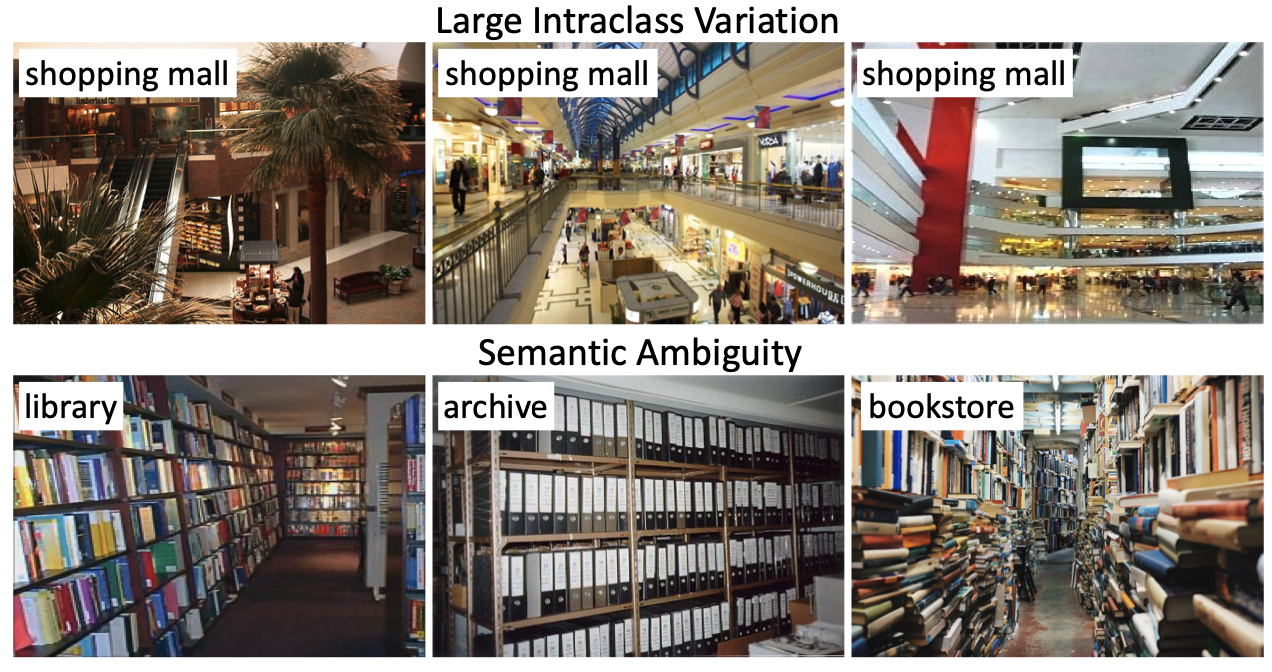
\includegraphics[width=\textwidth]{img/scene_class.png}
    \caption{Problem różnorodności wewnątrzklasowej oraz wieloznaczności semantycznej \cite{zeng2021deep}.}
    \label{fig:scene-class}
\end{figure}

Zadanie klasyfikacji sceny polega na przyporządkowaniu kategorii miejsca, w które przedstawia obraz. Istnieje duża różnica między klasyfikacja obrazka a klasyfikacją sceny. Klasyfikacja obrazka jako taka zajmuje się przyporządkowaniem klasy obiektu pierwszoplanowego, np. czy na obrazie znajduje się pies, czy kot. Klasyfikacja sceny natomiast musi wziąć pod uwagę wszystkie cechy obrazu, zarówno tła, jak i pierwszego planu, by określić odpowiednie miejsce. 

W kontekście środowisk wewnętrznych, klasyfikacja scen stanowi wyzwanie ze względu na zmienność scen wewnętrznych, obecność okluzji oraz fakt, że ten sam typ sceny może wyglądać inaczej na różnych obrazach. Wyróżniamy między innymi problem różnorodności wewnątrz klasowej oraz wieloznaczności semantycznej, co zostało przedstawione na rys. \ref{fig:scene-class}. Pierwszy z nich polega na fakcie, iż jedno miejsce może zostać przedstawione w bardzo różnej konfiguracji m.in. oświetlenia, ekspozycji, obiektów znajdujących się na obrazie. Drugi jest związany z występowaniem tych samych obiektów dla różnych klas scen.

\subsubsection{Segmentacja obrazu}
\begin{figure}[ht!]
    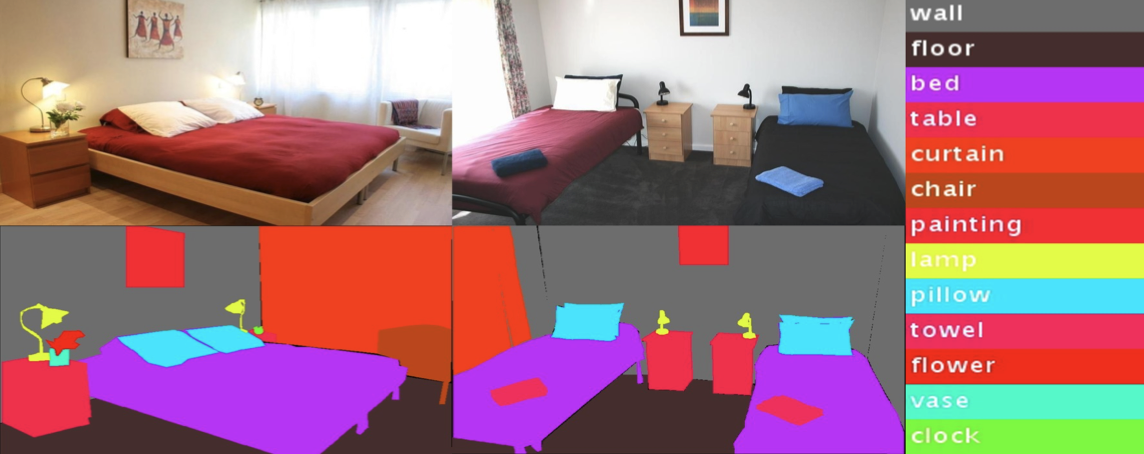
\includegraphics[width=\textwidth]{img/segment.png}
    \caption{Segmentacja wewnątrz pomieszczeń \cite{zhang2018context}.}
    \label{fig:segment}
  \end{figure}
  
Zadanie segmentacji obrazu to przyporządkowanie każdemu pikselowi etykiety takiej jak ,,łóżko'', ,,kanapa'' lub ,,umywalka'', do każdego piksela w obrazie (rys. \ref{fig:segment}). W rezultacie obraz zostaje podzielony na homogeniczne regiony pod względem pewnych własności. Segmentacja może być reprezentowana jako tablica 2D, gdzie każdy element odpowiada pikselowi w obrazie wejściowym i ma wartość wskazującą jego etykietę klasy.
  
Zadanie segmentacji można rozszerzyć do zadania segmentacji instancji (ang. instance segmentation), czyli segmentacji klasycznej rozszerzonej o rożróżnienie poszczególnych obiektów w ramach tej samej klasy. W przypadku klasycznej wersji nie jesteśmy w stanie rozróżnić dwóch stojących obok siebie łóżek, gdyż mapa segmentacji jest dla nich jednakowa. Segmentacja instacji pozwala natomiast takie rozróznienie uczynić. Segmentacja semtantyczna w dalszej części pracy będzie odnosić się do klasycznej wersji. Segmentacja instancji nie jest tematem pracy.
\subsection{Uczenie wielozadaniowe}
% # TODO